\chapter{Principal Component Analysis \& Statistical Shape \& Appearance Modelling}

\section{Introduction}

\subsection{Aims of Statistical Shape \& Appearance Models}

\subsection{General Methodology}

Generally SSAMs start with a rigid registration, where rotations and translations are applied to all meshes or models that form the input data set so that they share a common coordinate system.
Methods of performing the rigid registration often use an automated approach where certain degrees of freedom are restricted to ensure registration is achieved. 

\section{Measuring Vertebral Geometry}

Vertebral volume or the vertebral body volume may be the easiest and most obvious measure of geometric change within a set of vertebra. 
It has been shown in Chapter \ref{Chapter_HT} that there is a strong correlation between vertebral size and stiffness and so this may be enough for a range of comparisons between spines and individual vertebrae.
However, the input set of vertebrae contain a wide range of variation which can be seen visually, which may play an important role in the effect of cement augmentation and is another method of validating the outputs from the PCA generated set of models.

Measuring vertebral geometries in previous studies have either taken the measurements from x-ray scans \cite{Gilad1986,Gilad1985} or $\mu$CT scans \cite{Zhou2000,Cheung1994}, where the measurements have been made through the moving a cursor to the locations of specific points and reporting the distance between them.
While this method may produce accurate results, there is inherent human error associated, the number of measurements is limited to the number of planes available and applying this to large sets of data is time consuming which may lead to further error. 

The approach used here involves using the 1 mm voxel resolution models generated in ScanIP (v. 2016) which are are used for FE modelling.
The mask describing the vertebral body of these vertebrae is exported as a stereolithography file (STL), allowing the surface of the vertebra to be measured.
Measuring the vertebra was carried out in Matlab where the STL file was imported forming a point cloud describing the surface from the surface nodes.
Once imported the point cloud was split into thirds in each of the three anatomical planes, with the points describing the vertebra within these thirds being stored in nine array variables.
Cuboids were then fitted to the 3D arrays, maintaining the correct alignment and therefore prohibiting rotation of the cuboid.
The cuboid fits can be seen in Figures \ref{fig:cuboid_ax, fig:cuboid_sag, fig:cuboid_cor}.


\begin{figure}[ht!]
  \centering
  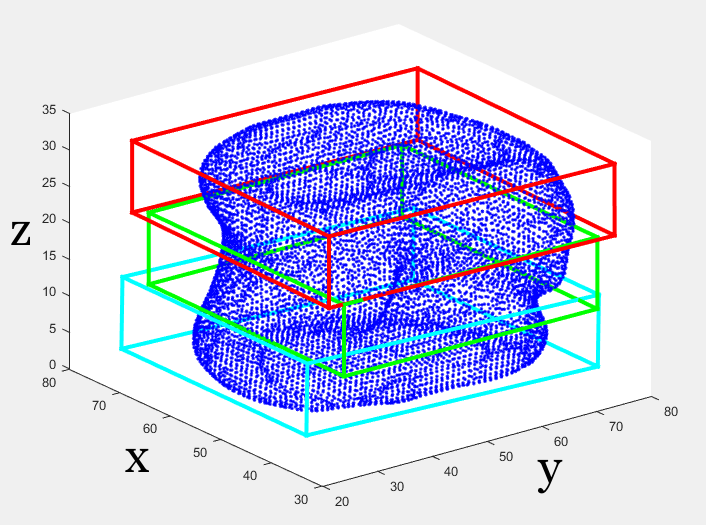
\includegraphics[width=4in]{Chapters/Chapter_PCA_images/Cuboid_fit_axial.png}
  \caption{The three cuboids fitted to the vertebra point cloud in the axial plane.}
  \label{fig:cuboid_ax}
\end{figure}

\begin{figure}[ht!]
  \centering
  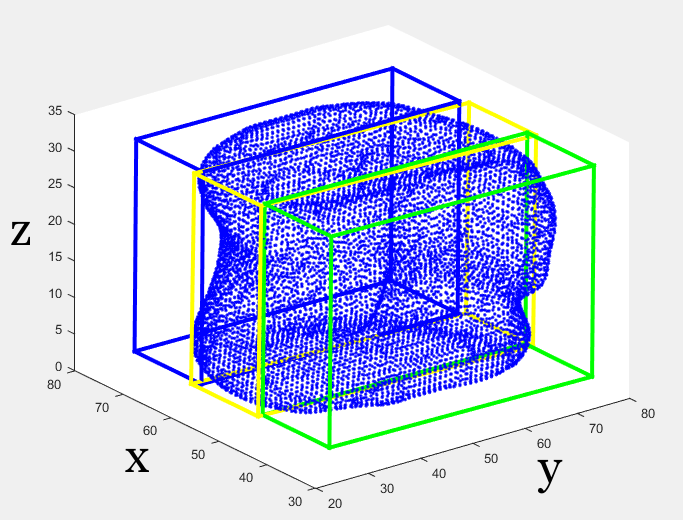
\includegraphics[width=4in]{Chapters/Chapter_PCA_images/Cuboid_fit_coronal.png}
  \caption{The three cuboids fitted to the vertebra point cloud in the coronal plane.}
  \label{fig:cuboid_cor}
\end{figure}

\begin{figure}[ht!]
  \centering
  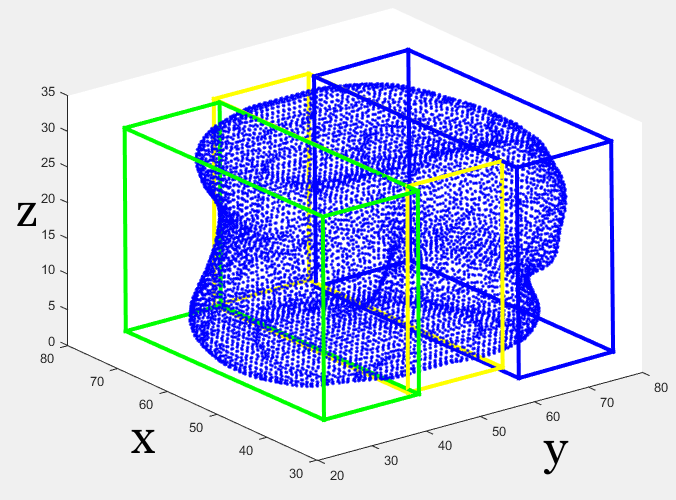
\includegraphics[width=4in]{Chapters/Chapter_PCA_images/Cuboid_fit_sagital.png}
  \caption{The three cuboids fitted to the vertebra point cloud in the sagital plane.}
  \label{fig:cuboid_sag}
\end{figure}

Measuring the two longer sides of the fitted cuboids gives a total of 18 measurements describing most aspects of the vertebral geometry.
This includes identifying wedge shaped vertebrae, recorded as reduced anterior height compared to the posterior height, left to right wedge shapes, recorded as sagital left height being smaller or larger when compared to the sagital right height. 

\section{PCA in ScanIP}

\subsection{Generating Vertebrae Models}



\subsection{Validating Generated Vertebrae}

\subsubsection{Geometry Validation}

Measuring the vertebral geometry 18 measurements

\subsubsection{Material Property (Greyscale) Validation}

\subsubsection{Resulting Stiffness Validation}


\subsection{Measuring \& Interigating Vertebral Variation}

\subsubsection{Geometry Variation}

\subsubsection{Greyscale \& Material Property Variation}

\subsubsection{Resulting Stiffness Variation}

\section{Effect of Injected Cement Volume, Shape \& Position}



\section{Effect of Injected Cement on Vertebral Variation}
